\chapter{Drátěné modely}

\begin{figure}[ht]
    \centering
    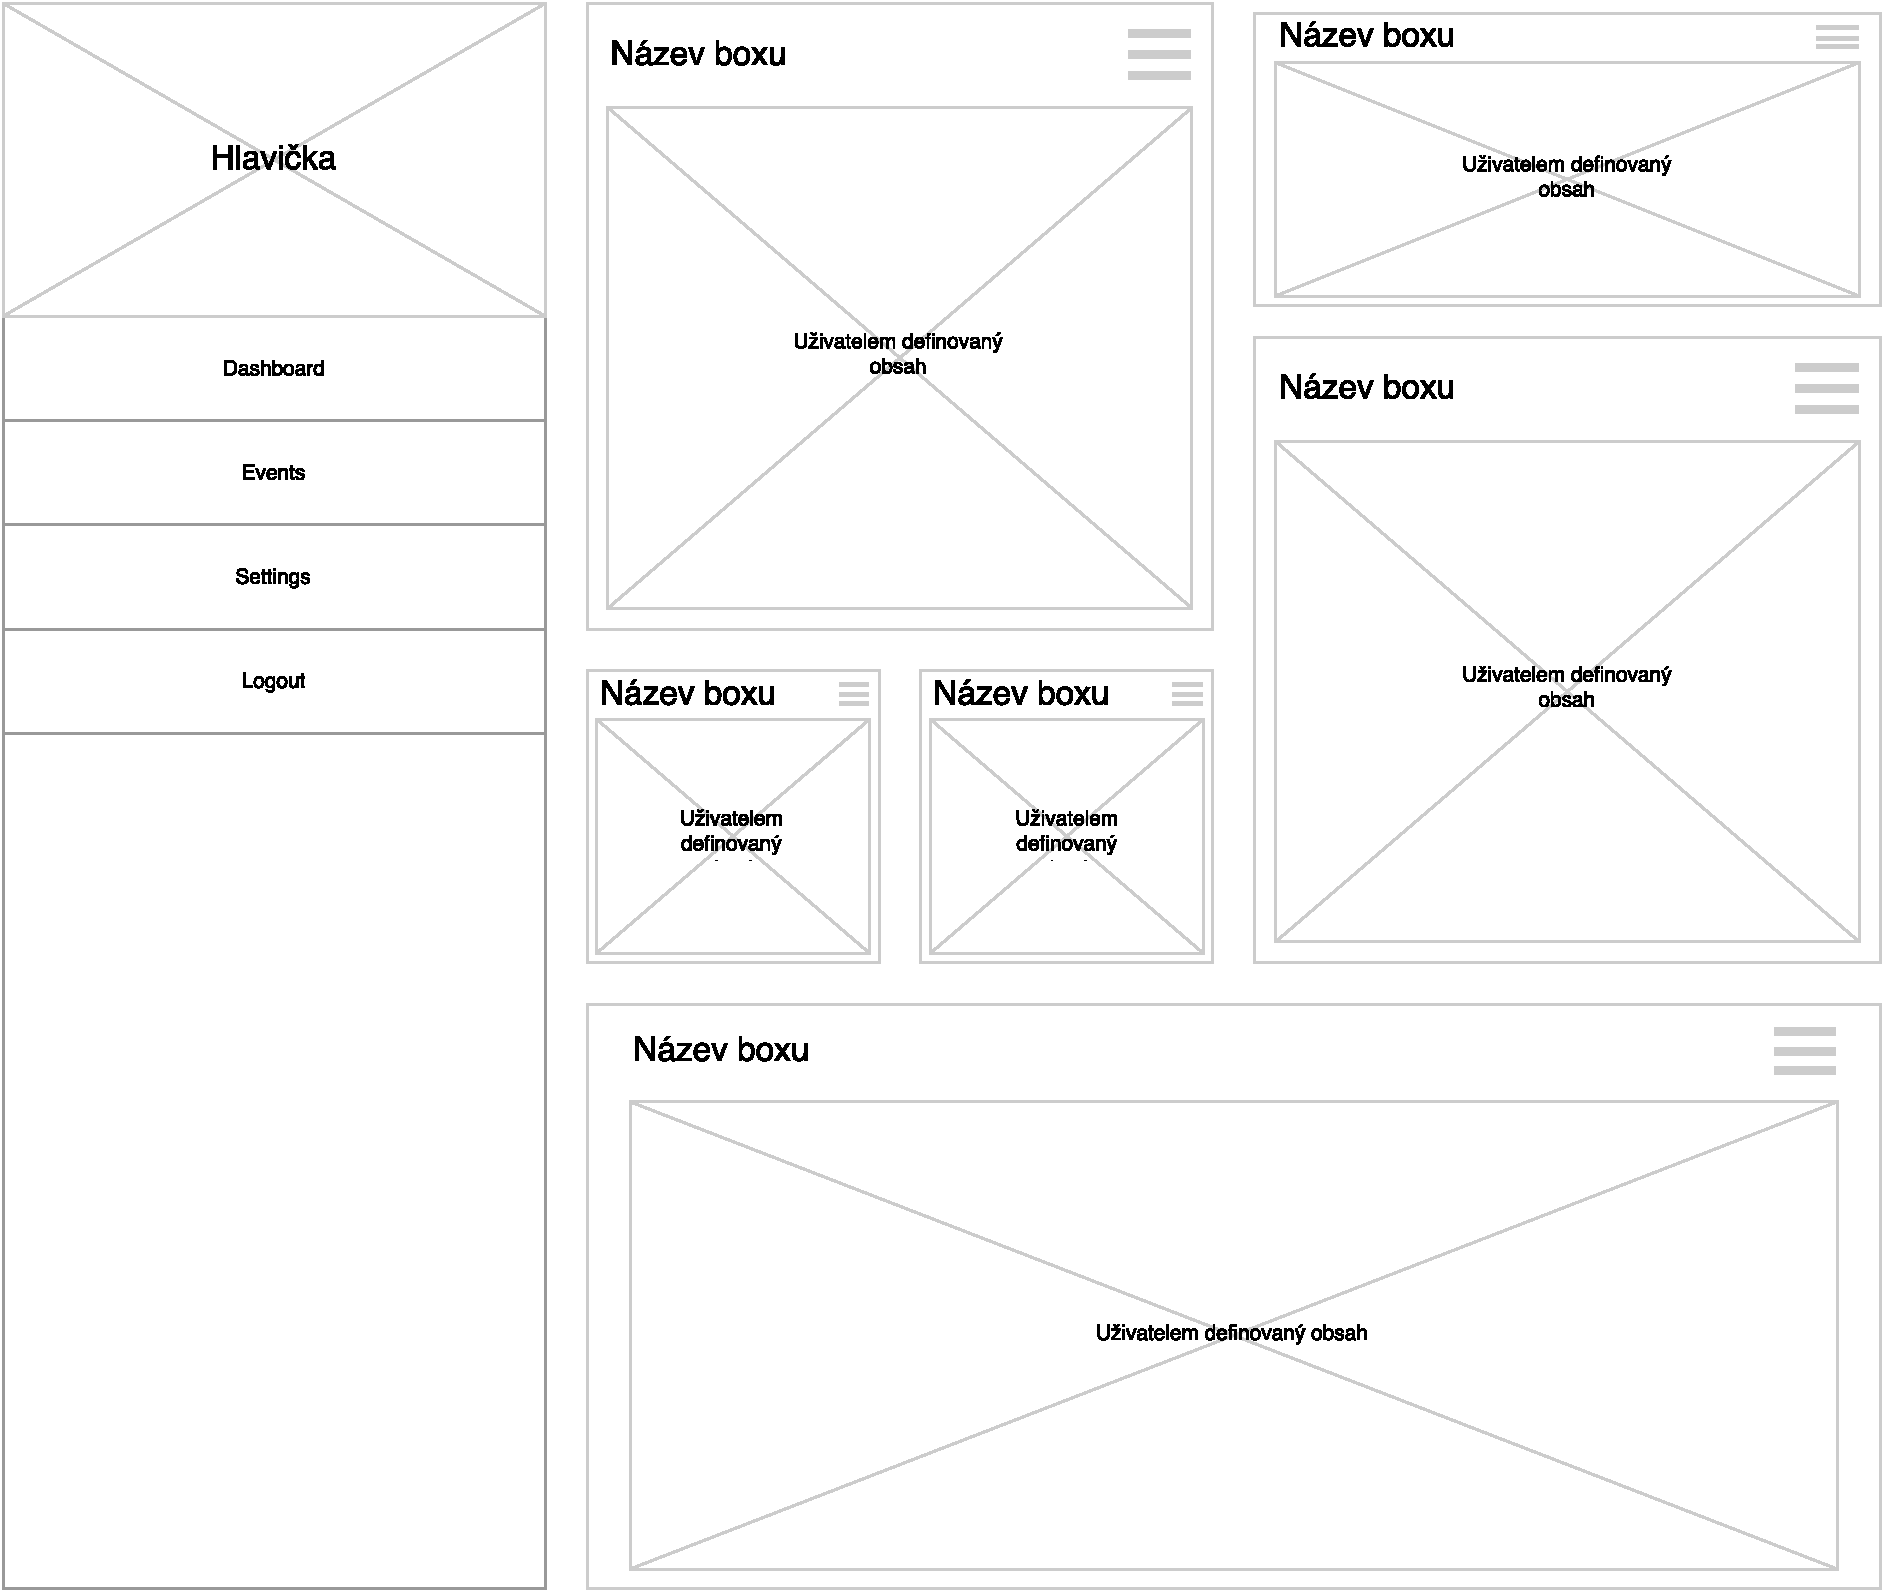
\includegraphics[width=1\textwidth]{fig/wf_dashboard.pdf}
    \caption{Drátěný model pro dashboard, který uživatel může konfigurovat.} \label{wf:dashboard}
\end{figure}

\begin{figure}[ht]
    \centering
    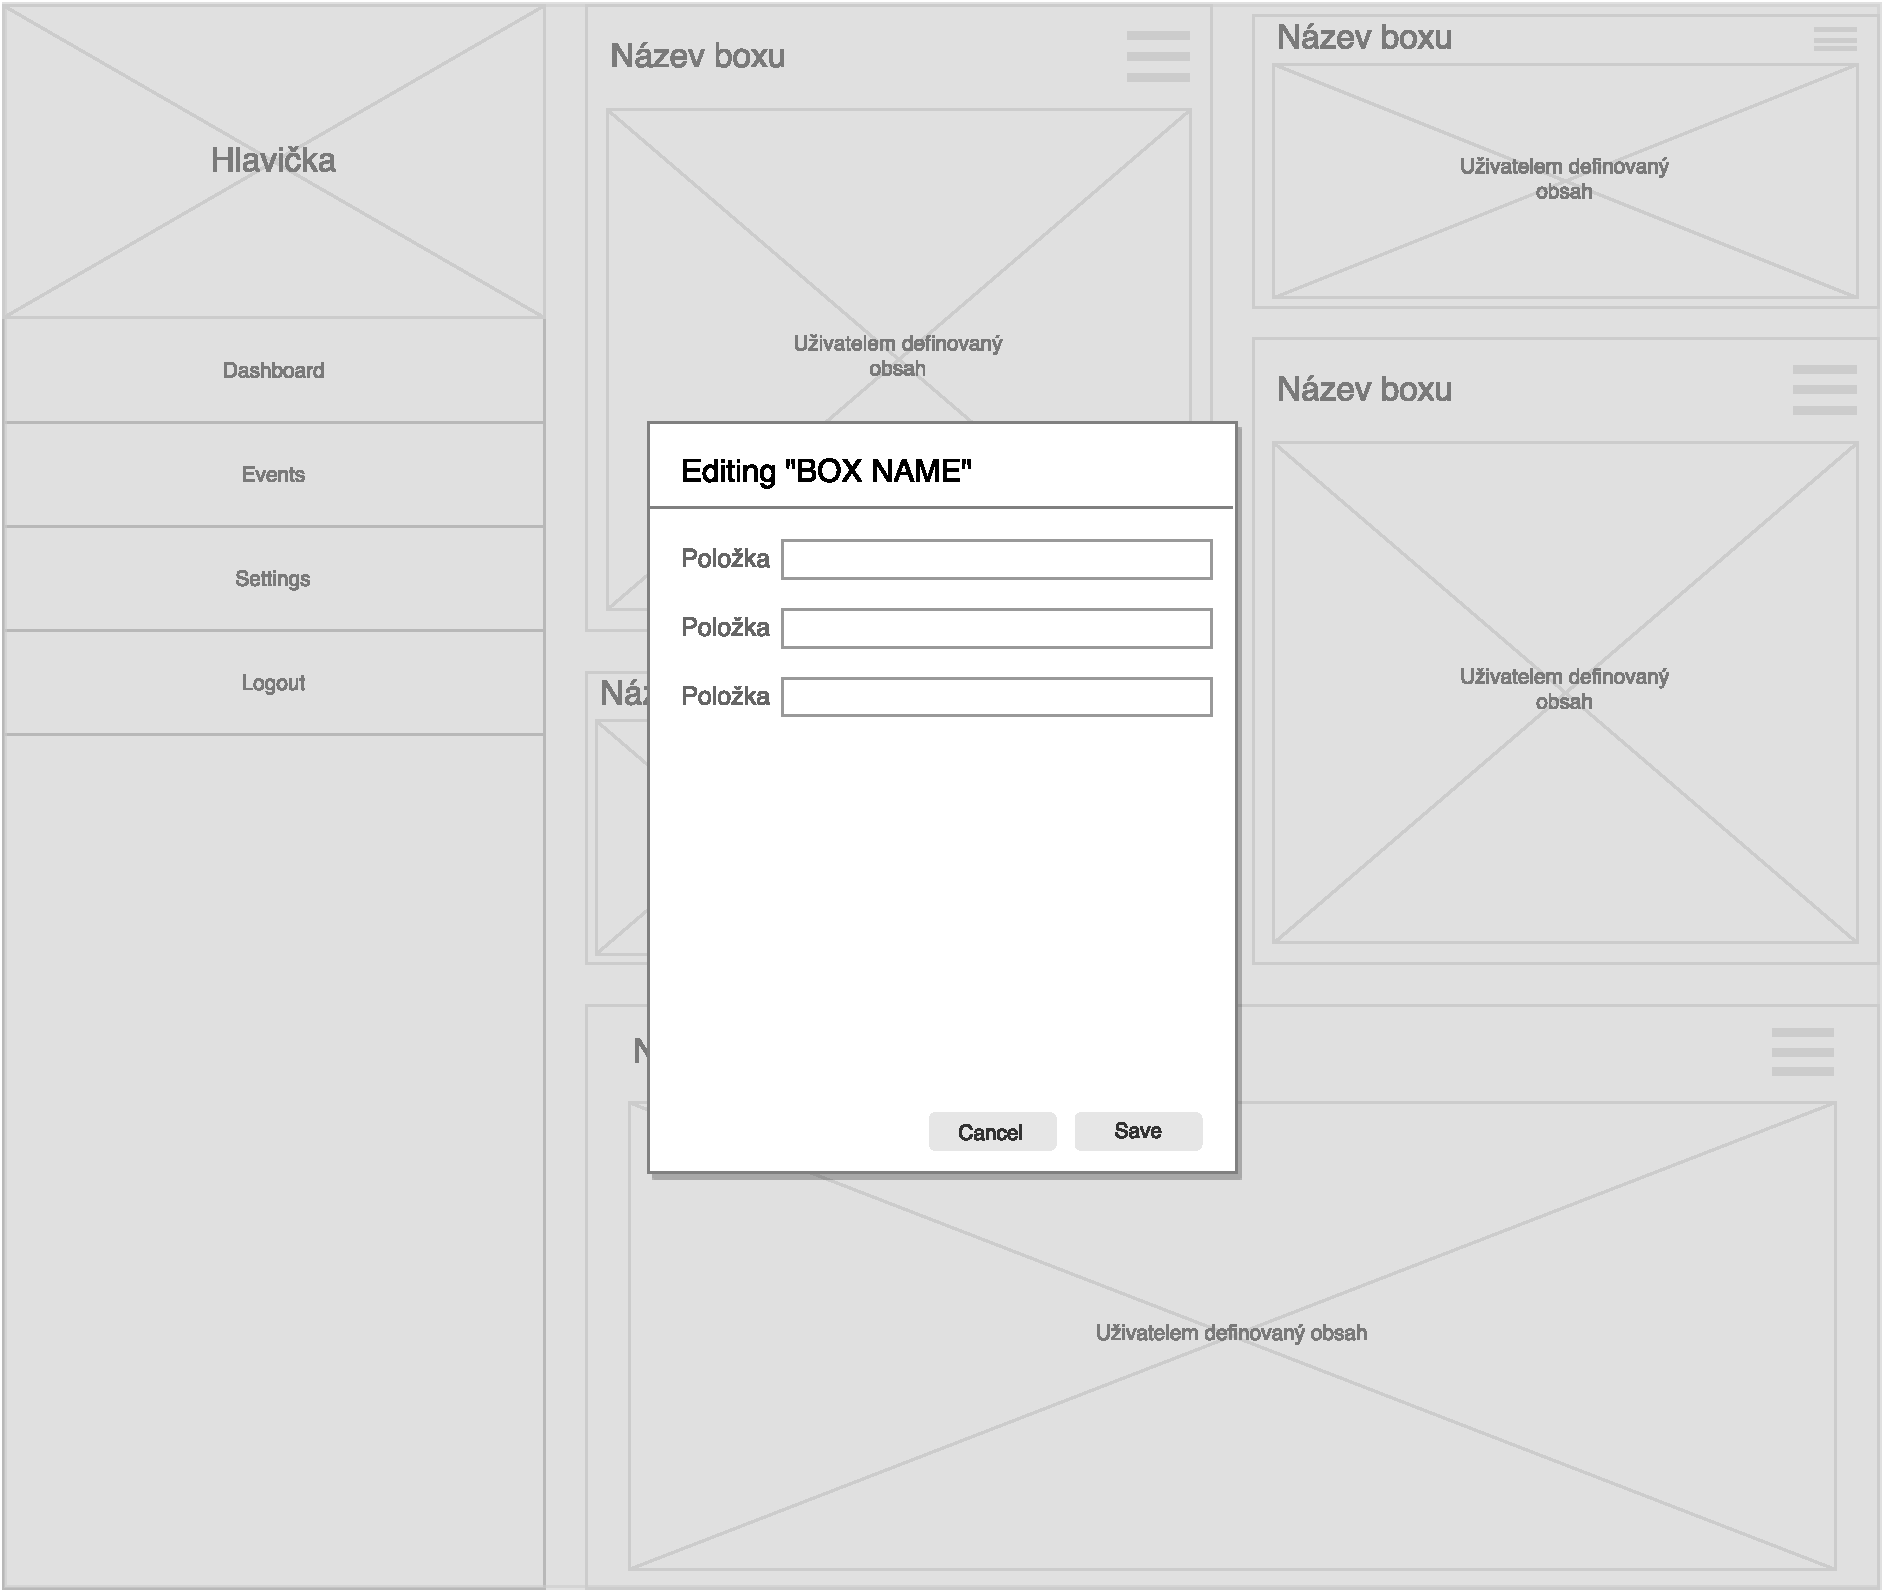
\includegraphics[width=1\textwidth]{fig/wf_dashboard_edit.pdf}
    \caption{Konfigurace boxu v dashboardu.} \label{wf:dashboard_edit}
\end{figure}


\begin{figure}[ht]
    \centering
    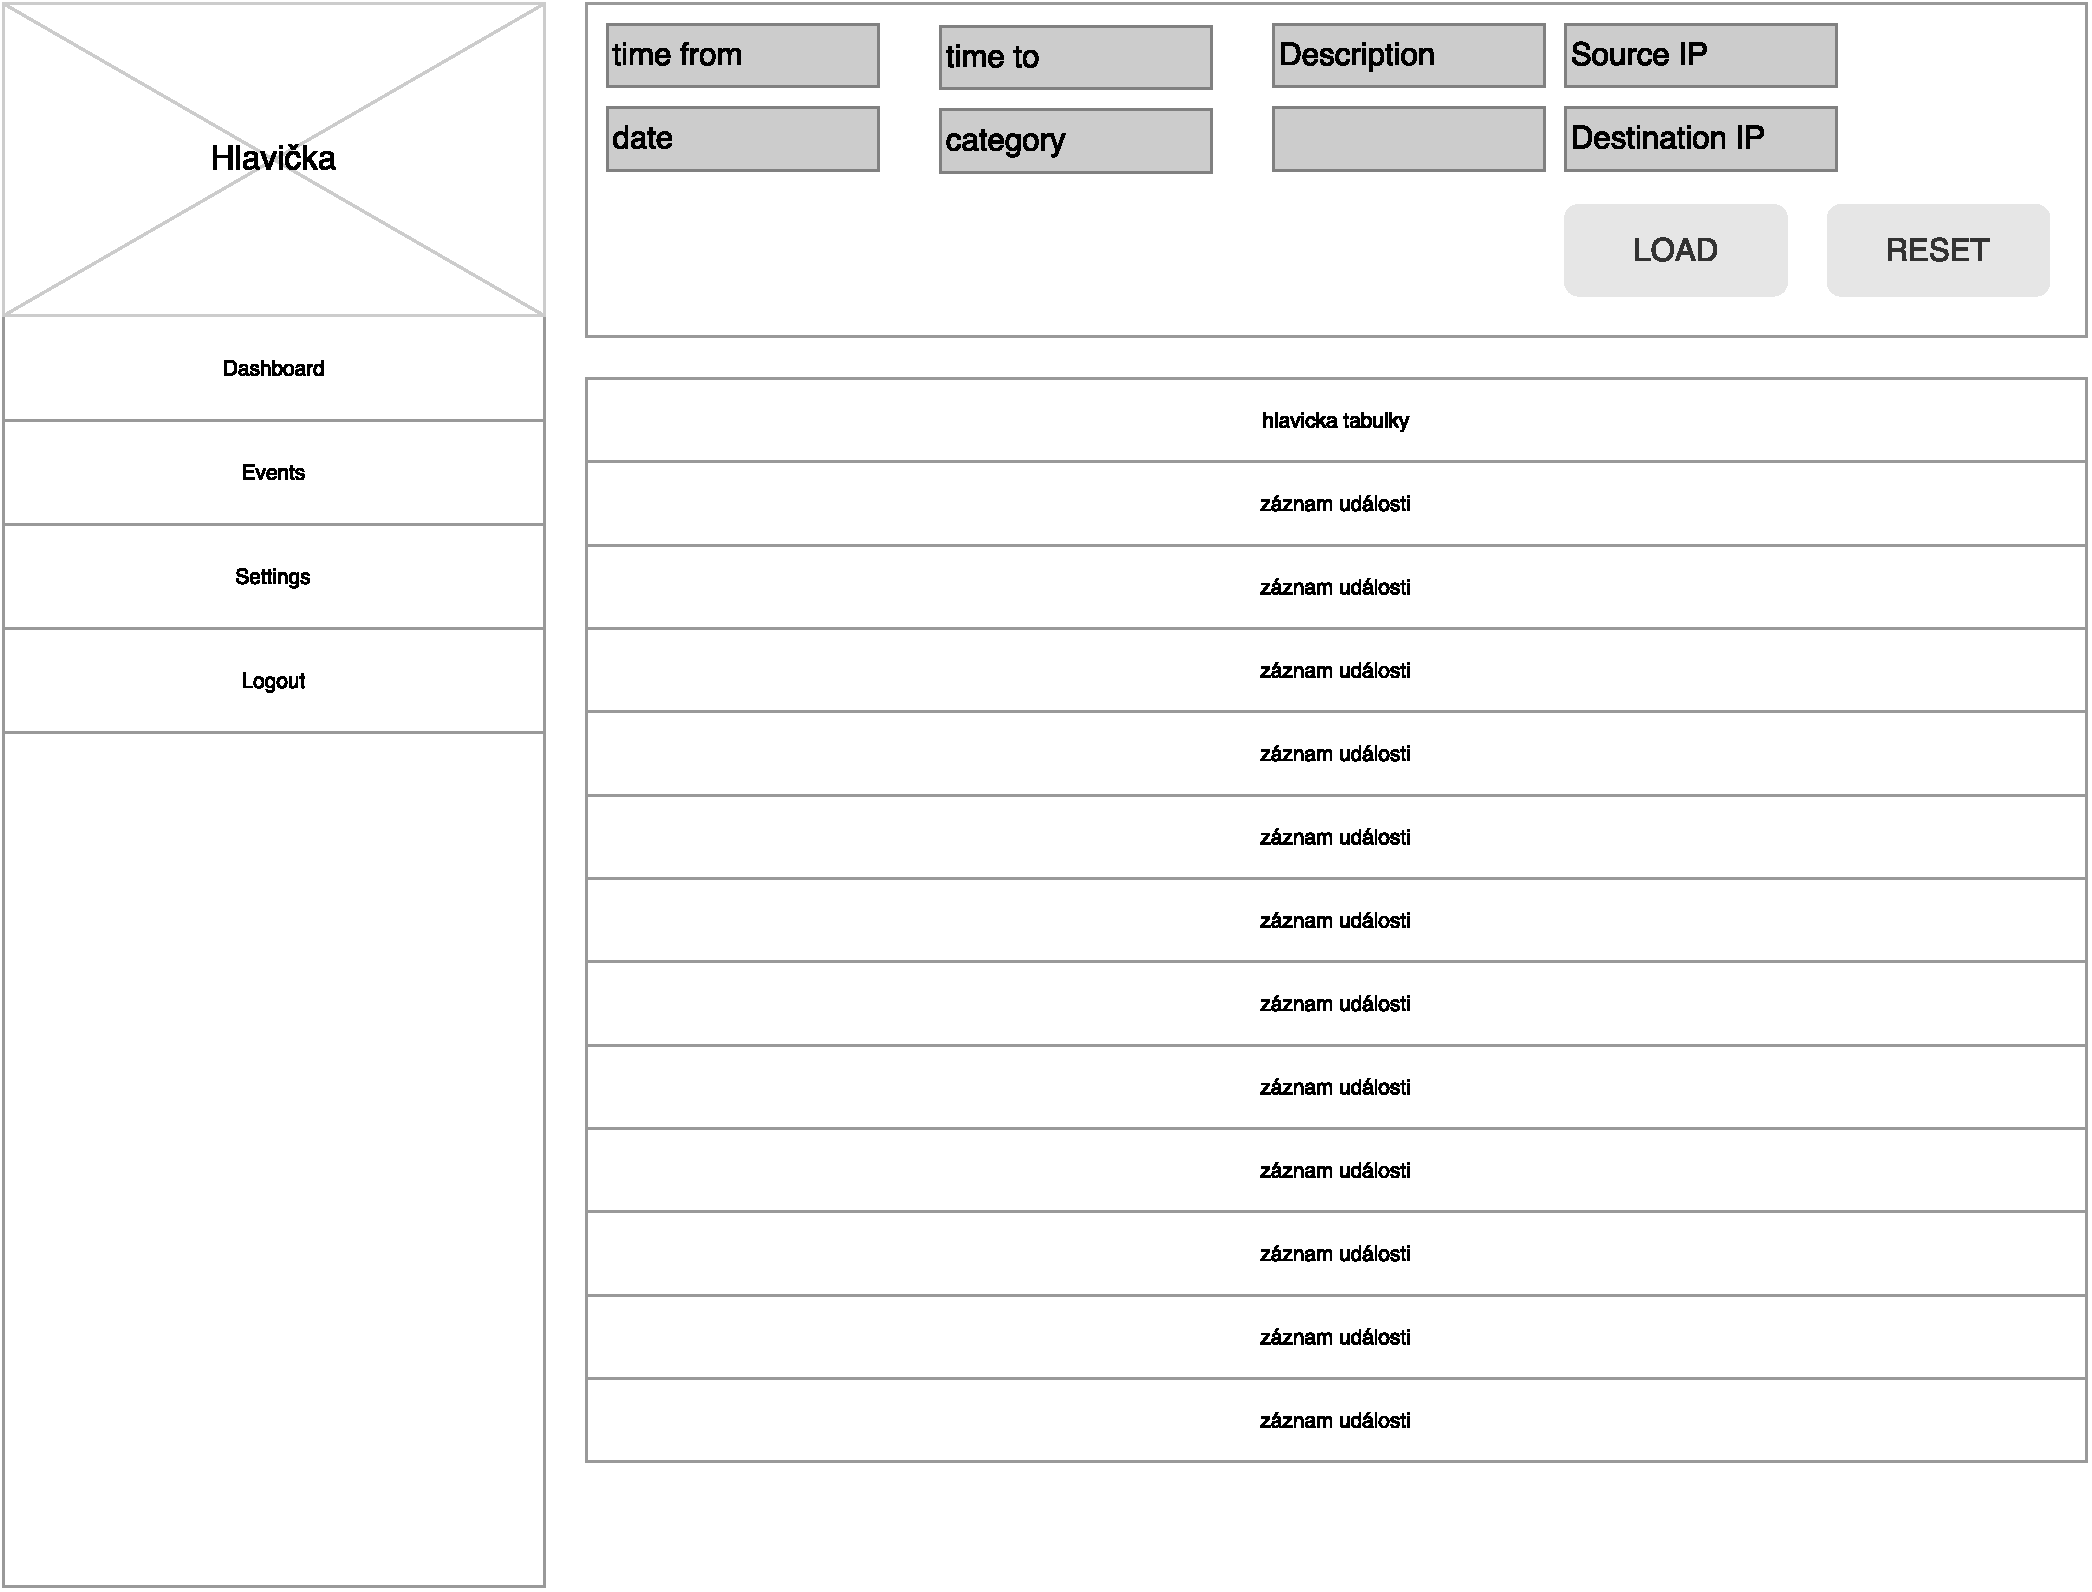
\includegraphics[width=1\textwidth]{fig/wf_dashboard_events.pdf}
    \caption{Přehled vyfiltrovaných událostí.} \label{wf:dashboard_events}
\end{figure}

\chapter{Seznam použitých Python knihoven}

\begin{figure}[ht]
\lstset{basicstyle=\small,style=JSON}
\begin{lstlisting}
Flask==0.10.1
Flask-Cors==2.1.2
itsdangerous==0.24
Jinja2==2.8
MarkupSafe==0.23
py-bcrypt==0.4
pycparser==2.14
PyJWT==1.4.0
pymongo==3.2
six==1.10.0
Werkzeug==0.11.3
\end{lstlisting}
\captionof{lstlisting}{Obsah souboru requirements.txt, který využívá nástroj pip pro instalaci Python knihoven.}
\label{code:requirements}
\end{figure}



\chapter{Obsah CD}
%\chapter{Manual}
%\chapter{Konfigrační soubor}
%\chapter{RelaxNG Schéma konfiguračního soboru}
%\chapter{Plakat}

